\chapter{Desarrollo}
\label{chap:desarrollo}
\vspace{0.5cm}

%%%%%%%%%%%%%%%%%%%%%%%%%%%%%%%%%%%%%%%%%%%%%%%%%%%%%%%%%%%%%%%%%%%%%%%%%%%%%%%%
% Objetivo: Exponer las partes relevantes de la implementación                 %
%%%%%%%%%%%%%%%%%%%%%%%%%%%%%%%%%%%%%%%%%%%%%%%%%%%%%%%%%%%%%%%%%%%%%%%%%%%%%%%%

\lettrine{S}e ha seguido un proceso de desarrollo en espiral con prototipado. El diseño y desarrollo de los diferentes componentes del sistema se presta a este tipo de ciclo ya que permite crear y probar en cada iteración un producto prototipo, centrándose en las primeras iteraciones en diseñar más e implementar menos y en las últimas solo refinar el software final. Cada iteración cuenta con una planificación de objetivos a alcanzar, detalles del trabajo y correcciones realizados, pruebas efectuadas y análisis de objetivos logrados en la iteración.

\section{Planificación y Presupuesto}

\section{Iteración 1}
\subsection{Planificación}
El objetivo de esta primera iteración es identificar los formatos, herramientas y componentes del proyecto, así como el diseño inicial de la arquitectura del proyecto, junto con el desarrollo del procesador de ficheros en formato MusicXML a hechos lógicos. Este primer paso tiene una fuerte carga de contextualización del trabajo de desarrollo así como la creación del espacio de trabajo en el que se sustenta todo el proyecto.

\subsection{Trabajo}
Como software de entrada para las partituras se escogió MuseScore, principalmente por ser \textit{opensource} y por su sencillez. MuseScore no posee una curva de aprendizaje difícil, ya que la introducción de las notas se puede hacer de forma visual en su interfaz mediante el ratón o con el teclado y no requiere mayor preparación para crear y exportar una pieza musical sencilla. Su soporte para \textit{plugins} también resulta interesante, ya que el proyecto podría llegar a transformarse en un \textit{plugin} para la herramienta si se desease una mayor integración con la misma. MuseScore además ofrece soporte para los tres formatos de ficheros musicales contemplados, así como para PDF y otros formatos finales de imagen.

Para el formato de entrada y salida, se compararon las propiedades de MIDI, LilyPond y MusicXML. Los tres formatos ofrecen posibilidades de edición, aunque cada uno sirve a un propósito diferente. MIDI no trabaja con ficheros textuales, sino que codifica de forma binaria toda la información de los eventos de la canción, LilyPond es un formato de texto plano pensado para que el usuario pueda editarlo a mano cómodamente, como si programase. Posee una estructura de marcado a través de etiquetas de solo apertura o autocerradas y trabaja con identaciones para formar la jerarquía del fichero, esto requiere al usuario escribir mucho menos, pero puede suponer problemas para un \textit{parser} convencional debido a que la identación de LilyPond no está estandarizada. Por último MusicXML se presenta como el formato idóneo para la tarea, ya que al ser una extensión de XML, está orientado a que una máquina pueda leerlo y crear una estructura en memoria con toda la información que necesita para poder extraer los datos de la partitura. Además, la implementación de un \textit{parser} de un lenguaje etiquetado como XML es un problema convencional y fácilmente abarcable.

En cuanto a la tecnología escogida para diseñar y construir el procesador de XML a ASP se optó por las bibliotecas Flex y Bison para C. EL principal motivo para ello fue que fueron las tecnologías empleadas en la asignatura Procesamiento de Lenguajes y durante una de las prácticas de la misma se desarrolló una primera versión de este mismo procesador que ahora se usa en el proyecto. Además Flex y Bison garantizan velocidad y eficiencia en el procesado. Por último pero no menos importante, y ya que el proyecto se está enfocando desde un punto de vista de desarrollo ágil, actualizar los ficheros de código de Flex y Bison es realmente sencillo, lo cual permitirá añadir nuevos elementos a reconocer cuando sea necesario.

Analizando la especificación del esquema de MusicXML de cara a desarrollar el \textit{parser} se identificaron las diferentes partes del mismo. MusicXML incluye información tanto musical como de representación gráfica de los diferentes elementos de la partitura. Todos esta información gráfica es generada automáticamente por el software que exporta el fichero MusicXML (MuseScore para el caso) y resulta irrelevante a la hora de extraer los hechos lógicos presentes en la partitura, por tanto se decidió obviarla. 

MusicXML declara inicialmente el número de voces presente en la partitura mediante la etiqueta part-list y sus etiquetas anidadas score-part. Más adelante, las etiquetas part se encargan de contener los compases mediante la etiqueta measure que a su vez contienen las etiquetas note. Son estas últimas etiquetas las que hay que desglosar para extraer los hechos lógicos, aunque la información de las etiquetas measure también es relevante, así como poder asignar un identificador a cada voz de la partitura para poder diferenciarlas a nivel lógico.

\begin{verbatim}
<note default-x="74.65" default-y="-25.00">
<pitch>
<step>A</step>
<octave>4</octave>
</pitch>
<duration>1</duration>
<voice>1</voice>
<type>quarter</type>
<stem>up</stem>
</note>
\end{verbatim}

La etiqueta note posee dos parámetros visuales, default-x y default-y,  que indican su posición en coordenadas x e y, como ya se ha comentado antes, esta información es meramente visual. La etiqueta pitch describe el sonido de la nota mediante el nombre de la nota usando notación internacional y la octava de la nota. Duration especifica la duración en tiempos del compás de la nota actual, voice asigna este sonido a la voz correspondiente, type indica la figura mediante el sistema fraccionario y stem dice si la plica de la nota es ascendente o descendente, de nuevo esto es meramente visual.

Ya que, inicialmente, el armonizador solo contemplará partituras uniformes (es decir, con un solo tipo de figura presente), unicamente necesitamos saber la voz, el compás, el tiempo en el que ocurre la nota relativo al compás y el sonido de la nota.

Con esta información en mente se procedió a desarrollar una versión actualizada del procesador de MusicXML a hechos en ASP. Se hizo uso de Flex para el análisis léxico y de Bison para el análisis sintáctico. El primer paso fue identificar los diferentes tags relevantes para el análisis léxico, estos son note para las notas, step para el ritmo, rest para los silencios, chord para los acordes, octave para la octava de cada nota, alteration para identificar sostenidos y bemoles, part para las diferentes voces de la pieza y por último elementos relevantes para el análisis de XML pero carentes de significado real para los hechos lógicos de la partitura tales como la apertura y cierre de etiquetas, campos textuales o símbolos varios.

En el código de Bison se diseñó la gramática primero y se integró junto con el código C encargado de tomar los datos extraídos por el \textit{parser} y exportarlos a un fichero de hechos lógicos listo para ser interpretado. La gramática diseñada para ello parte de una regla inicial que puede derivar en un bloque compuesto por etiquetas anidadas o en un error si el fichero no tiene el formato y estructura adecuados. La gramática inicial empleada fue la siguiente:

\begin{verbatim}
S : 		version doctype block | block
version : 	OPTAG QUES TEXT attr QUES CLTAG
doctype : 	OPTAG EXCL DOCTYPE doctags docurl CLTAG
doctags : 	/*...*/
TEXT doctags
docurl : 	/*...*/
KVOTHE TEXT docwords KVOTHE docurl
docwords : 	/*...*/
SLASHTAG docwords
TEXT docwords

block : 	OPTAG REST SLASHTAG CLTAG
OPTAG TEXT attr SLASHTAG CLTAG
OPTAG ALTER CLTAG TEXT OPTAG SLASHTAG ALTER CLTAG
OPTAG CHORD SLASHTAG CLTAG
OPTAG OCTA CLTAG TEXT OPTAG SLASHTAG OCTA CLTAG
OPTAG STEP CLTAG TEXT OPTAG SLASHTAG STEP CLTAG
part1 part2

part1 : 	OPTAG NOTE attr
OPTAG PART_ID KVOTHE TEXT KVOTHE
OPTAG TEXT attr

part2 : 	CLTAG body OPTAG SLASHTAG NOTE CLTAG
CLTAG OPTAG SLASHTAG TEXT CLTAG
CLTAG body OPTAG SLASHTAG TEXT CLTAG
TEXT EQUAL KVOTHE TEXT KVOTHE attr

body : 		body block
body TEXT
block
TEXT
\end{verbatim}

Los bloques de etiquetas se descomponen en tokens según su contenido o en dos partes (part1 y part2) dependiendo de si la etiqueta es autocerrada o no. Los errores que se pueden encontrar en este punto son que la etiqueta se abra pero no se cierre o que haya elementos de más no reconocidos tras la segunda parte de la misma. Las dos partes de cada etiqueta no autocerrada se corresponden respectivamente con la apertura de la etiqueta (part1) y con el contenido y cierre de la misma (part2). Por último se hace uso de una regla recursiva que permite anidar los bloques de etiquetas y contenido.

Se ha incluido en este procesador un par de opciones que pueden ser utilizadas en la llamada del mismo mediante línea de comando y que resultarían útiles más adelante. La opción -o permite especificar el nombre del fichero de salida resultante, mientras que la opción -s permite establecer una subdivisión arbitraria para las notas de la partitura.

\subsection{Pruebas}
Las pruebas realizadas al \textit{parser} revelaron que existía un problema de análisis al no poder verificar de forma sencilla que cada etiqueta se cerraba de modo correcto, es decir, que el nombre de la etiqueta que cierra un bloque sea el mismo del que la abrió, se implementó una pila en C para esta tarea. La implementación se realizó de modo que la pila no tuviese un tipo definido de partida, por flexibilidad, mediante el uso de punteros a void y el \textit{typecast} de los mismos en ejecución, aunque en el caso del \textit{parser}, solo se usó el tipo char*.

La implementación de la misma se hace mediante estructuras típicas de C enlazadas mediante punteros unidireccionales y el acceso a los datos de la pila se realiza mediante los conocidos métodos para operar con este tipo de datos (new, isEmpty, push, pop, etc.) 

Además de la adición de la estructura de pila para verificar esto se incluyeron más opciones de error en varias de las reglas gramaticales de modo que resultase más fácil la depuración del \textit{parser}. Esto reveló que había fallos en ejecución, ya que los resultados no eran los esperados. Este problema se debía a que la recursión se realizaba inicialmente mediante la posibilidad de que block derivase en otro block, así que se descompuso esta regla en un nuevo elemento body que añadía un paso más y abstraía los bloques de etiquetas y contenido pero a un nivel de granularidad algo más pequeño que \textit{body} en sí. Tras la inclusión de este paso intermedio, el \textit{parser} aún no terminaba de comportarse como era esperado y hubo que incluir reglas específicas para comprobar tags con formatos especiales tales como $<$?xml version$>$ o $<$!DOCTYPE$>$. Por último se comprobó que el \textit{parser} no contemplaba inicialmente tags autocerrados en su forma $<$tag$>$$<$/tag$>$ es decir, sin contenido. Al corregir estos detalles, cualquier pieza musical era transformada a hechos musicales a la perfección.

\begin{figure}
	\centering
	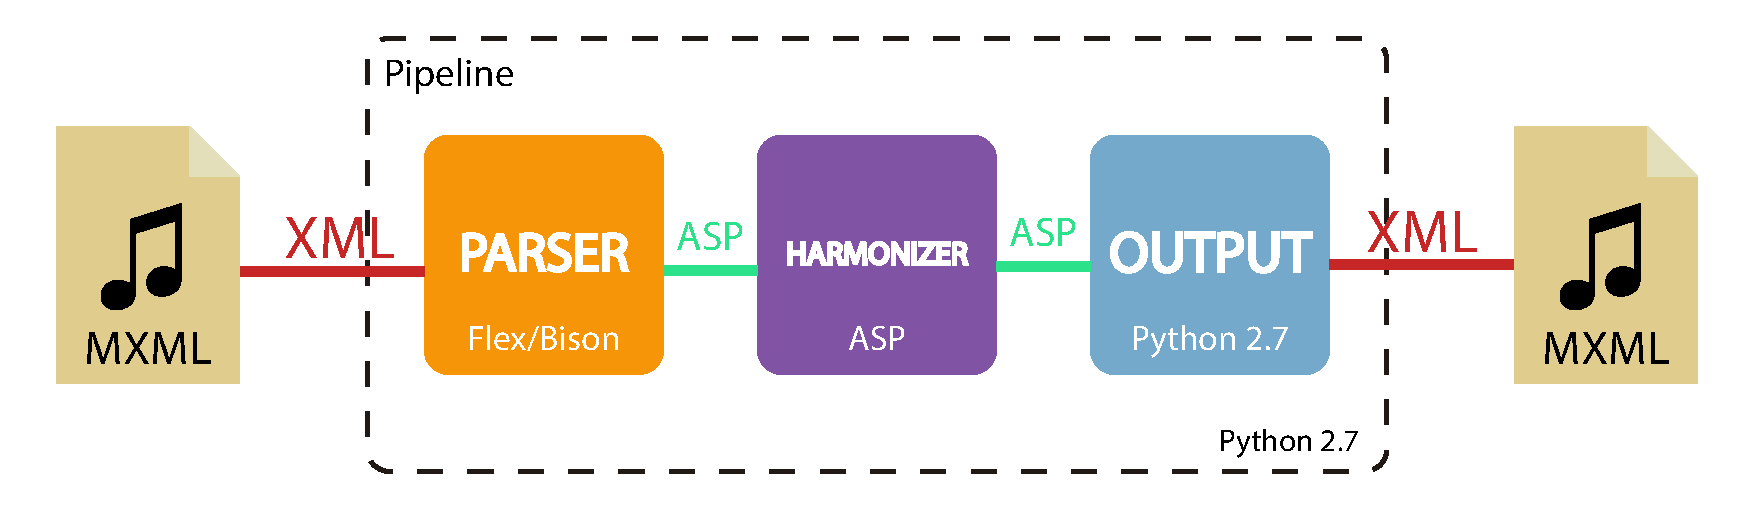
\includegraphics[width=0.8\linewidth]{imagenes/arquitectura_inicial.pdf}
	\caption{Diagrama del planteamiento inicial de la arquitectura del sistema}
	\label{fig:arquitectura_inicial}
\end{figure}

\subsection{Resultados}
En esta primera iteración se completaron todos los objetivos marcados en la planificación de la misma. Habiendo preparado correctamente el espacio de trabajo y definido bien los formatos sobre los que se trabajaría y habiendo implementado una primera versión del procesador de MusicXML a hechos lógicos.

\section{Iteración 2}
\subsection{Planificación}
El objetivo de esta iteración fue implementar una primera versión del pipeline que incluyese un módulo de armonización básica en ASP. Para ello se fijaron una serie de restricciones que simplificaban algunos problemas detectados durante el análisis. Inicialmente no se tendrán en cuenta las notas adyacentes en la partitura ni subdivisiones de las mismas, no obstante y de cara a futuras iteraciones, se establece una figura base como período de análisis horizontal de la melodía y una figura base de subdivisión, aunque para esta iteración ambas se establecerán a negra (\textit{quarter note}) de modo que se asignará el acorde correspondiente a cada golpe rítmico de la partitura teniendo en cuenta las múltiples voces que la componen de manera vertical.

\subsection{Trabajo}
Se modificó el procesador de MXML a ASP y se ha incluido una opción para subdividir la partitura de forma automática en base a la nota más breve de la partitura o forzar toda la partitura a un solo tipo de figura omitiendo aquellas figuras de menor duración, aunque esto lleve a resultados incorrectos musicalmente. La salida deseada y el formato de entrada para el módulo de procesado ASP usan el formato "note(voz, tono, tiempo)" siendo voz el número de la voz que interpreta la nota, tono un valor numérico asociado a la nota, no en frecuencia sino calculado como el número semitonos a partir de una nota base A0, es decir, el La más grave que puede interpretar MIDI; y tiempo la posición de la nota en la partitura.

Para el desarrollo del módulo de procesado ASP se sigue el proceso conocido como \textit{Generate and Test}, muy habitual en el paradigma. Como su nombre indica, consta de dos partes: generación y prueba. En la generación se usan reglas que definen todas los resultados posibles del problema para después, en la fase de prueba, restringirlos mediante reglas que prohíben total o parcialmente ciertas combinaciones al exponerse a hechos lógicos aportados por el procesador de MXML a ASP. Esta metodología se usó desde el principio en cada iteración a partir de la presente para desarrollar la parte en ASP correspondiente ya que aunque las reglas de generación permanecerán intactas, estas serán revisadas por si fuera necesario cambiarlas o añadir alguna regla nueva.

En esta primera aproximación, las reglas de generación establecen los posibles acordes que compondrán la solución y se realiza una asignación acorde-unidad rítmica (como ya se comentó, la unidad rítmica base inicialmente será la negra) en base a las notas presentes para un instante dado en cada voz. Para realizar esto es necesario interpretar cual es el grado de cada nota presente en la escala de la pieza, (de nuevo, por restricciones iniciales se considera Do mayor) ya que de este modo podremos especificar una serie de reglas que abstraigan el hecho de qué nota suena en si y lo sustituyan por qué grados aparecen en cada momento dado de la partitura, pudiendo deducir así qué acorde es el más correcto de entre todas las posibilidades, a más notas presentes de la escala correcta, menos posibilidades, de aparecer notas no pertenecientes a la escala, no se podrá resolver el acorde y el programa se detendrá con un error.

La fórmula empleada para derivar los grados de la escala es $[(valor-base) mod 12]$ siendo valor el valor númerico asignado a la nota y base la nota de la que se parte para calcular los grados. Esta expresión resulta en los semitonos de distancia entre la nota base y la nota actual. La operación de módulo es necesaria para abstraer la octava a la que pertenece la nota, aunque más adelante esto pueda ser un hecho relevante. Con una comparación directa del valor obtenido con una distribución dada según el modo (Mayor o Menor) de la escala es posible asignar los grados correspondientes a cada nota. Por último se generan hechos que indican cuantas voces toman parte en la pieza, así como los tiempos en los que suena al menos una nota.

Se crearon dos ficheros a mayores que especifican los acordes a considerar, otorgándole un nombre en notación numérica romana y creando múltiples predicados que especifican qué grados de la escala pertenecen a dicho acorde. De este modo no es necesario especificar en ningún momento cuantas notas tendrán los acordes con los que se trabaje, y aunque principalmente se trabajará con acordes de tres notas, esto permitiría ampliar la complejidad en el futuro al incluir acordes de dos o cuatro notas. Teniendo en cuenta los posibles acordes, y mediante una restricción de cardinalidad, se generan todas las soluciones iniciales, haciendo que solo se asigne un acorde a cada tiempo en el que suena al menos una nota. A mayores se especifica una restricción de integridad que anula cualquier solución en la que, para un tiempo en el que esté presente una nota concreta, el acorde asignado en la solución comprobada no contenga esa nota. 

A mayores se ha incluído como parte de esta iteración, el diseño e implementación de un pipeline en python que automatice las llamadas al procesador MXML a ASP y al módulo de armonización. En este primer prototipo se implementó una pequeña funcionalidad de interpretación de la salida del módulo ASP a un vector de soluciones. En futuras iteraciones, se añadirá más funcionalidad a dicho pipeline, como más opciones de entrada o diferentes representaciones de las soluciones ofrecidas por el módulo ASP haciendo uso de alguna librería que permita representar de nuevo la partitura en el formato deseado. El pipeline agrega y combina las diferentes opciones de los módulos a los que llama, en este caso se incluyeron únicamente las opciones -n, que especifica a clingo cuantas soluciones mostrar, y -m, encargada de alternar entre los modos de armonización mayor y menor. El pipeline no contepla aún opciones relacionadas con el módulo de procesado ya que la opción -s incluida en la anterior iteración está fijada a 1 por las restricciones especificadas para este prototipo. 

//// Incluir diagrama de secuencia

\subsection{Pruebas}
Se han realizado pruebas individuales a los módulos de procesado y armonización, además se han realizado pruebas al pipeline creado, sirviendo de este modo de pruebas de integración de los diferentes módulos y de la herramienta al completo.

Para el procesador se han probado múltiples ficheros de entrada así como las distintas opciones que contempla. No presenta problemas para ficheros MusicXML estándar generados por Musescore y programas similares, ante la ausencia de fichero, ficheros incompletos, ficheros XML que no sean MusicXML o ficheros que directamente no sean XML el procesador detiene la ejecución y produce el mensaje de error adecuado en cada caso. En cuanto a las tres opciones que presenta esta primera versión, la opción de ayuda -h detiene la ejecución independientemente de la presencia de otros parámetros y muestra el modo de uso del módulo parser por sí solo, la opción para especificar el fichero de salida -o funciona correctamente en cualquier caso, excepto cuando el directorio especificado para almacenar el fichero de salida no existe. En la siguiente iteración se planteará la posibilidad de dejar esto de este modo intencionadamente o si forzar la creación de los directorios necesarios. Por último la opción de subdivisión -s, que para este primer prototipo ha de ser especificada manualmente o dejada en su valor por defecto funciona para cualquier valor. Esto no es del todo correcto ya que la subdivisión solo debería ser posible para potencias de 2, en el segundo prototipo se corregiría esto.

El módulo de armonización no presenta una gran complejidad de prueba ya que solo depende del fichero de entrada. Si este no está presente no produce resultado alguno, y en caso de estarlo y no ser correcto, produce un resultado de insatisfacibilidad. En caso de existir alguna solución esta es correctamente devuelta por pantalla. Las diferentes piezas probadas, pese a ser sencillas por las limitaciones de este primer prototipo, ofrecieron resultados de armonización correctos.

Por último, en las realizadas para el pipeline se analizaron las diferentes opciones y casos de entrada de la herramienta. Ante los casos erróneos donde el módulo de procesado fallaba y no generaba fichero LP de salida, el pipeline no detenía la ejecución y llamaba al módulo ASP igualmente, aunque este fallaba al no tener un fichero de hechos lógicos con el que funcionar, no obstante el pipeline si que debería comprobar esto y por tanto se corrigió. Con ficheros de entrada adecuados el pipeline realizaba una ejecución completa y recogía los resultados ofrecidos por el módulo ASP, ofreciendo por pantalla una representación más amigable así como un resultado de satisfacibilidad. La opción -m (alternar entre modo mayor y menor) funcionaba como se esperaba, restringiendo los dos posibles valores de la opción a los especificados (major o minor) y deteniendo la ejecución en caso de encontrar un valor incorrecto, mientras que la opción -n (número de soluciones exploradas) restringe también correctamente los valores de N a únicamente enteros y no hace falta mayor comprobación ya que cualquier valor entero es válido como opción para el módulo ASP. Ambas opciones producían el efecto deseado en la ejecución del pipeline.

\subsection{Resultados}
Este primer prototipo se completó en dos semanas, siendo los mayores problemas de la iteración la falta de soltura con el paradigma y el lenguaje, así como detalles técnicos de falta de librerías y software. Se logró implementar una versión inicial del pipeline junto con una temprana pero funcional versión del módulo de armonización.


\section{Iteración 3}

\subsection{Planificación}
El objetivo de esta iteración es completar el desarrollo de un segundo prototipo de la herramienta que incluya las siguientes mejoras:
\begin{itemize}
	\item Subdivisión real y automatizada de las notas de la pieza a la longitud de la nota mínima presente en la partitura
	\item Especificación en el pipeline de la longitud del tiempo de análisis horizontal
	\item Inclusión de la posibilidad de realizar análisis horizontal en ASP
	\item Flexibilización de los resultados del módulo de armonización, es decir, en vez de prohibir las soluciones erróneas, se anotarán los errores en la partitura y se escogerá aquella solución que minimice el número de errores
\end{itemize}
Además se incluirán en este prototipo las correcciones a los errores de ejecución de los módulos no corregidos en el primero.

\subsection{Trabajo}
Se modificó el \textit{parser} substancialmente ya que este imprimía a un fichero según procesaba las notas. Esto no planteaba problema alguno si la subdivisión se especificaba de antemano mediante el parámetro correspondiente, pero sí que resultaba complicado mantener esta aproximación si la unidad de subdivisión debía calcularse al mismo tiempo que se procesaba la partitura en MXML. Se plantearon dos soluciones, o bien incluir en el pipeline en python un análisis previo a la conversión de MXML a hechos en ASP que dedujese cual era la nota de menor longitud y la usase como parámetro en la llamada al \textit{parser} o bien se modificaba el comportamiento del anterior para realizar simultáneamente ambas tareas. 

Se optó por la segunda opción por motivos de coherencia con el sistema, es decir, no incluir funcionalidad innecesaria y replicada en el pipeline, cuya tarea es simplemente manejar las entradas y salidas de los diferentes módulos, y por motivos de eficiencia, ya que como se ha mencionado no hay necesidad de procesar el mismo fichero dos veces, siendo una de ellas en un lenguaje interpretado en vez de compilado, lo que añadiría un sobrecoste temporal evitable.

Los cambios implementados en el \textit{parser} implicaron principalmente incluir un nuevo tipo de dato nota para almacenar la información de las notas de la partitura y una nueva pila que contuviese las notas extraídas del MXML. Una vez procesado todo el fichero de entrada, hallada la nota más breve y almacenadas las notas en la pila, ésta se vacía y se imprimen en el fichero de hechos lógicos de salida teniendo en cuenta la subdivisión pertinente, bien sea esta la calculada o la especificada por parámetro. En caso de especificar una subdivisión no válida, es decir, de mayor longitud que alguna de las notas presentes en la partitura, se imprime por pantalla un mensaje de error y la nota no es subdividida. Esto produce comportamientos no deseados a la hora de realizar la deducción de la armonía, ya que es necesario trabajar siempre con piezas con notas de longitudes iguales a lo largo de toda la partitura.

El módulo de armonización incluye una nueva constante que indica la longitud del intervalo de tiempo mínimo de análisis armónico horizontal, a su vez es posible especificar en la llamada al módulo el valor de esta constante. Se ha modificado, por tanto, la regla que restringe las posibles soluciones para analizar en dichos intervalos de tiempo. Además dicha regla se ha suavizado y en vez de ser una restricción de integridad, esta activa un nuevo predicado error(voz, grado, tiempo) que indica los grados erróneos presentes en la partitura que no encajan con el acorde asignado para la solución. Posteriormente se realiza un proceso de optimización consistente en la minimización de el número de estos predicados de error, es decir, aquellas soluciones con menor número de errores serán las óptimas. Además en caso de no encontrar una solución con cero errores, los errores aparecen también en la salida para que el usuario pueda conocer qué tiempos contienen notas equivocadas.

Se han incluido en el pipeline opciones tanto para indicar al \textit{parser} una subdivisión específica como para indicar al módulo de armonización el intervalo horizontal de armonización. Se han implementado en el pipeline, con vistas al futuro de módulo de salida, una serie de clases para almacenar los resultados y poder devolverlos más tarde en el formato más conveniente. Error y Chord son clases para almacenar y representar los acordes asignados en la solución así como los errores presentes en la partitura, es decir, aquellas notas que no encajan con los acordes asignados. A su vez, HaspSolution es una clase orientada a almacenar y representar soluciones completas incluyendo una colección de objetos Chord y otra de objetos Error, así como el grado de optimizazión de dicha solución. Por último, la clase ClaspResult almacena la salida sin procesar de una ejecución del módulo ASP, aunque cuando esta es instanciada, dicha salida se procesa y se crean una colección de objetos HaspSolution conteniendo sólo aquellas soluciones que alcancen un cierto valor de optimización. La relación entre las clases así como sus métodos se detallan en \textbf{el diagrama de clase pertinente}.

\subsection{Pruebas}
Se han continuado con las pruebas a los diferentes módulos, dando por válidos los resultados de las pruebas de la anterior iteración se procedió a probar las nuevas funcionalidades de cada módulo.

En el \textit{parser} se comprobó que la autosubdivisión funcionaba correctamente al introducir partituras con diferentes longitudes de notas, además en caso de forzar una subdivisión incorrecta se producía el mensaje de aviso adecuado explicando el problema. Si la subdivisión forzada era correcta funcionaba como debía. El nuevo tipo de datos, nota, así como la pila para almacenar las diferentes notas de la partitura fueron probados junto con esta nueva funcionalidad, ya que fueron implementados expresamente para su funcionamiento.

En el módulo ASP se probaron piezas más y menos complejas, algunas creadas de forma artificial para producir errores y se vio que el nuevo análisis funcionaba y detectaba dichos errores, no obstante seguía produciendo soluciones válidas marcando aquellas notas erróneas.

En cuanto al pipeline se comprobó que las nuevas opciones en la llamada a éste funcionasen correctamente, ya que las dos nuevas opciones son simplemente parámetros que se pasan más adelante al módulo \textit{parser} o al módulo ASP, bastó con realizar una comprobación de validez del valor pasado en la llamada. Se probaron además las cuatro clases de almacenamiento de las soluciones diseñadas e implementadas para este prototipo, siendo ClaspOutput la única que tuvo que ser probada más exhaustivamente ya que es la que realiza el procesado de la salida del módulo ASP, el resto simplemente cuentan con constructores y funciones de representación textual. 

\subsection{Resultados}

\section{Iteración 4}

\subsection{Planificación}
El objetivo de esta iteración es crear un tercer prototipo que busca no sólo refinar la armonización como el anterior si no ampliar funcionalidad de la herramienta. Se busca incorporar un módulo de salida escrito en python al cual el pipeline se encarga de pasarle los datos formateados correctamente para que dicho módulo, haciendo uso del toolkit \textbf{music21}, exporte al formato deseado. 

\subsection{Trabajo}
El módulo ASP se ha aumentado para incluir generación de notas en un número de voces adicionales que puede ser especificado por parámetro. Además se creó un fichero de conversiones encargado de traducir valores de notas a grados, octavas y viceversa. De este modo los grados generados durante el procesado de la partitura pueden ser traducidos de vuelta a un valor de nota para que el módulo de salida llamado desde el pipeline reconstruya la pieza. Para la generación de notas en las nuevas voces se ha impuesto una única restricción fuerte, que dos notas consecutivas no realicen un salto melódico de dos octavas o más, mientras que mediante predicados de minimización se controla la cantidad de saltos de una quinta realizados por una misma voz. Junto con estas adiciones, se han incluído dos nuevos acordes a la lista de posibles acordes deducidos por el módulo, siendo estos la subdominante séptima (IV7) y la dominante séptima (V7) tanto de los modos mayor como menor.

Se ha diseñado implementado una nueva clase de almacenamiento Note y se ha incluido un método a HaspSolution que transforma una solución al tipo de dato requerido por el \textit{toolkit} music21 para producir los diferentes formatos de salida.

Se ha optado por incorporar \textbf{music21} al módulo de salida principalmente por la cantidad de formatos con los que puede trabajar, tanto en entrada como en salida, y aunque lo ideal será exportar un fichero MusicXML, la idea de poder generar PDF, MIDI o Lilypond resulta más que atractiva. Este módulo toma un objeto ClaspResult como entrada y haciendo uso del método de una de los objetos HaspSolution contenidos en él, representa dicha solución en el formato adecuado.

En el \textit{pipeline} se ha incluido una opción para especificar el número de voces adicionales que deben ser añadidas y otra opción para especificar el formato de salida. Este componente ahora se encarga también de llamar al módulo de salida.

\subsection{Pruebas}

\subsection{Resultados}

\section{Iteración 5}
\subsection{Planificación}
El cuarto prototipo tiene como objetivo tener en cuenta los tiempos débiles y fuertes de la partitura para refinar ciertas preferencias ya incluidas anteriormente o posibles nuevas preferencias basadas en dichos tiempos. Para esto será necesario modificar el módulo ASP, el \textit{parser} y el pipeline. Además se busca refinar el módulo de salida para ajustar la representación en partitura de la solución e incluir mejoras visuales. Como en los anteriores, este prototipo corregirá los errores detectados en el anterior.

\subsection{Trabajo}
En el parser se han incluido dos nuevas funciones principales: análisis de medida de compás y reconocimiento de silencios "verdaderos" y silencios completables. La primera atiende a la necesidad de indicarle al módulo ASP la métrica del compás para poder identificar tiempos débiles y fuertes, mientras que la segunda atiende a la carencia de una manera sencilla de representar en música con un símbolo aquellos huecos que siendo silencios en la partitura original deben ser completados por el módulo ASP y no ser tratados como silencios en sí. Para la métrica del compás, se implementó en el \textit{parser} la capacidad de itentificar las diferentes métricas de compases así como el tiempo en el que ocurren, aunque por comodidad y sencillez, se ha asumido que un cambio rítmico en el compás debe ocurrir en todas las voces a la vez. Esto crea predicados "measure(T,N)" que indican para un tiempo T, el número N de figuras que componen el compás. No es necesario especificar la subvidisión ya que esta se fija y normaliza durante el análisis de la partitura. De este modo, aunque el compás fuese un 4/4 (compases de cuatro negras), si la subdivisión detectada y empleada es de corchea, será traducido a 8/8 (compases de ocho corcheas). Para los silencios "verdaderos" y los silencios completables se ha optado por una solución relativamente sencilla no solo de identificar por el \textit{parser} sino también fácil de usar por el usuario final de la herramienta, mediante la notación de letras de la pieza, se pueden indicar en cada voz los intervalos de tiempo en los cuales los silencios deben ser tratados como completables. Para ello solo hace falta escribir los símbolos "[" y "]" al principio y final del intervalo respectivamente.

Gracias a las mejoras implementadas en el \textit{parser}, el módulo ASP puede diferenciar tiempos débiles de tiempos fuertes, así como los intervalos que debe completar. Se han definido acordemente varios predicados nuevos, como busybeat(V,B) siendo B un tiempo de la voz V que indica aquellos tiempos en los que inicialmente ya hay una nota o silencio, todos aquellos beat(B) que no son busybeat(V,B) son freebeat(V,B), y deben ser completados. Además se han definido los predicados $strong_beat(B)$, $semistrong_beat(B)$ y $weak_beat(B)$ que corresponden a los tiempos fuertes, semifuertes y débiles de cada compás en la partitura. Gracias a esto se han creado predicados que matizan los diferentes errores de la partitura $error_in_strong(V,G,B)$, $error_in_semistrong(V,G,B)$ y $error_in_weak(V,G,B)$ que definen en qué tipo de tiempo ocurren los errores de la pieza y permite minimizarlos con diferentes prioridad (a más fortaleza de tiempo, más prioridad). Por último y para dar más flexibilidad en la búsqueda de la armonización correcta se ha incluído el acorde de dominante séptima (V7) en los modos mayor y menor.

El módulo de salida se ha refinado para representar mejor las notas incluyendo información del tipo de compás, clave y duración de las figuras. Además se colorean en rojo los errores detectados y se anotan en los tiempos adecuados los acordes inferidos por el módulo ASP.

Por último, el pipeline cuenta con una nueva opción timeout que permite especificar un tiempo máximo de búsqueda del óptimo en el módulo ASP, ya que para piezas largas, el espacio de búsqueda crece muchísimo y es necesario poder limitar el tiempo de ejecución. Además, al final de la ejecución, y tras enumerar todas las soluciones escogidas por el módulo ASP, permite al usuario escoger qué solución exportar o mostrar, teniendo por defecto la última, ya que se supone más refinada.

\subsection{Pruebas}

\subsection{Resultados}

\section{Iteración 6}
\subsection{Planificación}
 En esta iteración se perfeccionarán algunas funcionalidades de los diferentes módulos y se añadirá un sub-módulo de preferencias melódicas al ya creado módulo ASP. El quinto prototipo busca ser, esencialmente, una mejora del anterior.

\subsection{Trabajo}
Para facilitar la entrada de silencios que representan huecos completables por el módulo ASP se ha cambiado el enfoque, y se ha abandonado el delimitado de secciones completables con corchetes en las letras de la canción por suponer algunos problemas al no poder ubicar dichas letras en tiempos en los que haya un silencio, por claridad y por no interferir con las posibles letras de una partitura real no creada ni modificada textit{ad-hoc} para el programa. MusicXML permite marcar elementos de la partitura como no visibles, esto solo afecta a la hora de imprimir en papel dicha partitura y a nivel musical no interfiere con ningún elemento. Además, la visibilidad de una nota o silencio puede ser facilmente alterada en cualquier editor de partituras desmarcando una casilla al clicar sobre dicho elemento, lo cual facilita mucho el marcado de estos tiempos completables. Esto se reflejó en el \textit{parser}, que en vez de contemplar los dos símbolos utilizados anteriormente, ahora solo tiene que comprobar la visibilidad de un elemento para determinar si asignar un tiempo completable a dicho tiempo.

Para refinar la subdivisión en tiempos débiles y fuertes, se reimplementaron tanto en el módulo ASP como en el \textit{parser}, esto fue debido a que no es sencillo establecer dichos tiempos aritméticamente solo teniendo en cuenta la cantidad de notas del compás, sino que también se ha de tener en cuenta el tipo y subdivisión del compás con respecto a la nota de referencia usada para armonizar. Para esto es importante no normalizar el compás leído en el fichero XML y generar nuevos predicados indicando los valores del compás sin modificar. En el módulo ASP se ha incluido, de modo similar a los acordes, una tabla de tipos de compás y su subdivisión teniendo en cuenta el compás y la longitud del tiempo de armonización. Se han incluido en dicha tabla los compases más habituales, pero de nuevo, al igual que con los acordes incluidos en los ficheros correspondientes, pueden ser ampliados si el usuario lo necesitase. Una vez inferido el tipo de subdivisiñon del compás, calcular los tiempos débiles y fuertes se puede realizar de forma aritmética, de modo similar a como se hacía en el prototipo anterior. Debido a la pérdida de información resultante de uniformizar las notas de la partitura no es posible detectar los subtiempos fuertes y débiles dentro de secuencias de corcheas, semicorcheas, etc. Además se ha optado por descartar la inferencia de tiempos semifuertes ya que solo añadían complejidad a la búsqueda del óptimo y no aportaban mejores resultados, los que en el prototipo anterior eran semifuertes, en este son directamente tiempos fuertes.

Se creó un sub-módulo ASP de preferencias melódicas que busca alcanzar una optimización mayor a la hora de generar nuevas voces o cubrir tiempos completables con algunas mejoras que atienden, principalmente, a la secuencia de notas de una misma voz. Se ha definido el salto melódico de forma genérica y éste es minimizado en notas consecutivas usando el tamaño del salto como peso a la hora de minimizarlo, con esto se logra una melodía más continua y sin saltos erráticos, al mismo tiempo que se limita el espacio de búsqueda considerablemente. Se ha inferido un nuevo predicado tendencia que analiza, dado un par de notas de una voz, si la tendencia melódica es ascendente, descendente o no varía. Además se ha definido otros predicados relacionados que analizan si la tendencia entre dos voces diferentes es la misma o si es contraria, maximizando estos predicados se consigue un ligero efecto de imitación de tendencia entre voces.

Se estudió la posibilidad de incluir también en este sub-módulo de preferencias melódicas la detección de patrones secuenciales armónicos y melódicos comunes como las secuencias de sextas, que siguen un determinado patrón de saltos melódicos en cada voz y que sería interesante completar de forma correcta para buscar una mayor naturalidad en las líneas melódicas de la pieza a la hora de completarla. Para implementarlo se ha incluido en el módulo una asignación de acordes a tiempo con su propia detección de errores (aunque estos acordes y errores no se representan en la salida). Con estos acordes se pueden analizar los saltos armónicos presentes entre las diferentes voces de la partitura y deducir la inversión del acorde. Solo se trabaja con las inversiones primera y segunda por sencillez, ya que solo se busca el enlace entre estos acordes. Dentro de las dos posibles segundas inversiones solo se tiene en cuenta a su vez la  de cuarta y sexta, por ser la más usada en enlaces armónicos. Posteriormente se maximiza el enlace entre la primera y segunda inversión o entre segundas inversiones consecutivas.

Se ha descartado la detección de apoyaturas con el fin de no contemplarlas como errores por un motivo similar, al uniformizar la longitud de las figuras de la partitura, no es posible detectarlas bien, ya que una de las características de las apoyaturas es que "roban" brevemente el tiempo fuerte a una nota representativa del acorde de la armonía. Para detectar dicha brevedad sería necesario conservar la longitud original de las notas, lo que imposibilitaría una armonización correcta.

En el módulo de salida se ha incluido la representación mediante nombre del acorde y no mediante el numeral romano.

En el pipeline se ha incluido una nueva opción -M que permite activar o desactivar este módulo de preferencias melódicas a gusto del usuario. Además la llamada al módulo de salida produce un objeto de partitura music21 que puede ser manejado de diferentes modos según nuevos parámetros, -f permite especificar el formato de salida (Principalmente PDF, MIDI o XML) siempre y cuando se disponga de herramientas en el PC para generar dicho formato. Por otra parte, usando la opción -S se puede pedir al pipeline que no genere un fichero nuevo, si no uno temporal para mostrar o reproducir al terminar la ejecución. La opción -o permite especificar el nombre del fichero, de no estar presente, tomará el mismo nombre que el del fichero MusicXML de entrada

\subsection{Pruebas}
Módulo de preferencias melódicas falla por los enlaces de sextas, se revisa en la siguiente iteración.
Algunas piezas dan problemas por VoiceChords

\subsection{Resultados}

\section{Iteración 7}
\subsection{Planificación}
En esta iteración se busca mejorar el módulo de procesado para que sea capaz de extraer más información y metadatos de la partitura original y así conseguir una salida más fiel. Además se busca incluir en este mismo módulo la auto-detección de la clave de la partitura basándose en la armadura presente. A mayores se busca un modo más conveniente de incluir voces de una determinada tesitura a la partitura. Como en otras iteraciones se busca corregir los fallos encontrados en las pruebas de la anterior.

\subsection{Trabajo}
Se incluyeron en el \textit{parser} nuevos \textit{tokens} y reglas en la gramática para poder extraer metadatos y otra información de la partitura y exportarlos a un fichero temporal usado por el módulo de salida. Los diferentes datos extraídos para cada partitura son:
\begin{itemize}
	\item \textbf{title:} Título
	\item \textbf{composer:} Compositor
	\item \textbf{base\_note:} Longitud de la nota más breve presente
	\item \textbf{key\_name:} Nombre de la clave en la que se armonizará la pieza
	\item \textbf{mode:} Modo (mayor o menor)
	\item \textbf{last\_voice:} Número que identifica cual es la última voz presente
\end{itemize}
Los dos primeros atienden a una cuestión estética, simplemente sirven para que el módulo de salida disponga de esta información y pueda completarla a la hora de reconstruir la partitura. Los tres siguientes son datos relevantes para el módulo de armonización, mientras que el último sirve para añadir voces nuevas correctamente a la partitura. 

El procesador extrae una nueva pieza de información de la partitura, conocida como "figure". Figure en la forma "figure(voice,duration,beat)" es un hecho lógico que describe la duración de una figura para un pulso de una voz dada. De este modo, pese a subdividir las notas a la longitud de la más breve para el análisis, se pueden recomponer en la salida fidedignamente. Además esta nueva información puede usarse en la generación de nuevas notas en la pieza.

Los nuevos datos extraídos por el procesador son leídos desde el pipeline y son pasados a los subsiguientes módulos de armonización y salida respectivamente. Se ha modificado el parámetro -v del pipeline y su efecto en el resto de módulos. En vez de especificar una cantidad de voces a añadir, toma como mínimo un argumento indicando la tesitura (por nombre) o el rango de notas para las nuevas voces. El pipeline se encarga de crear, a partir de los datos de este parámetro -v un nuevo fichero temporal "extra\_voices.lp" que será incluido en la llamada del módulo de armonización para que dichas nuevas voces se tengan en cuenta. Se ha añadido un parámetro -k que permite especificar, mediante la letra de la nota base de la escala, la clave en la que está escrita la pieza, de no ser especificada esta se calcula automñaticamente, como ya sucedía con el parámetro -d usado para especificar la longitud fraccionaria de la nota en la cual se debían subdividir todas las de la partitura.

En el módulo de armonización se ha incluido un nuevo archivo similar al de acordes o tipos de compases que describe las diferentes tesituras de las voces presentes en la partitura. Este documento es ampliable al igual que los mencionados para incluir nuevos instrumentos o tesituras. Se han definido los principales tipos de voz coral (tanto masculinos como femeninos) y sus rangos de notas más frecuentes. 

\begin{center}
	\begin{tabular}{ | l | c | c | }
		\hline
		Tesitura & Nota mínima & Nota máxima \\ \hline \hline
		Bajo & 40 & 64 \\ \hline
		Barítono & 45 & 69 \\ \hline
		Tenor & 48 & 72 \\ \hline
		Contra-Tenor & 52 & 76 \\ \hline
		\hline
		Contralto & 53 & 77 \\ \hline
		Mezzo-Soprano & 57 & 81 \\ \hline
		Soprano & 60 & 84 \\ \hline
	\end{tabular}
\end{center}

Además el módulo de armonización tiene en cuenta los nuevos hechos "figure" y los utiliza para generar correctamente las secciones a completar. Es decir, si se especifica un patrón en los tramos a rellenar, las nuevas notas generadas seguirán dicho patrón. Para las voces nuevas donde no existen dichos patrones se asigna la nota más breve ya que crear patrones rítmicos es muy costoso computacionalmente se estudia la posibilidad de crearlos mediante un postprocesado en el módulo de salida en futuras iteraciones. Se ha eliminado la constante "extra\_voices" al funcionar de un modo diferente la inclusión de voces nuevas en la partitura. Para este mismo módulo se corrigió el archivo de preferencias de enlace de sextas, ahora separado del archivo de preferencias melódicas.

Se ha definido una nueva clase "VoiceChord", que representa un acorde realizado por un solo instrumento polifónico ya que los este tipo de acordes producían fallos en la anterior iteración.

En el módulo de salida se han corregido algunos errores encontrados en las iteraciones anteriores y haciendo uso de los nuevos predicados "figure" se puede reconstruir la partitura mucho mejor que antes. Además el módulo de salida tiene en cuenta y representa correctamente el nuevo elemento "VoiceChord" y la partitura además se escribe en la clave especificada o detectada por el procesador.

El pipeline cuenta con una opción nueva -6 que permite incluir la preferencia de los enlaces de sextas, que pese a estar corregida, sigue siendo muy costosa por tener que realizar una armonización a tiempo independientemente del intervalo de armonizacion fijado.

\subsection{Pruebas}
Todo bien excepto generación de notas nuevas.

\subsection{Resultados}

\section{Iteración 8}
\subsection{Planificación}
La última Iteración que cierra el ciclo de desarrollo busca corregir los problemas encontrados durante las pruebas de la anterior iteración, al ofrecer unos resultados relativamente malos en cuanto a tiempo de ejecución al incorporar secciones a completar en la partitura. Además tiene como objetivo incluír la posibilidad del uso de ficheros de configuración que alteren el comportamiento del módulo de armonización ajustando los diferentes pesos de las preferencias a maximizar o minimizar.

\subsection{Trabajo}


\subsection{Pruebas}

\subsection{Resultados}

